\documentclass[11pt,a4paper, table]{article}
% Useful packages, sorted so packages of similar functionality are grouped together. Not all are essential to make the document work, however an effort was made to make this list as minimalistic as possible. Feel free to add your own!

% Essential for making this template work are graphicx, float, tabularx, tabu, tocbibind, titlesec, fancyhdr, xcolor and tikz. 

% Not essential, but you will have to debug the document a little bit when removing them are amsmath, amsthm, amssymb, amsfonts, caption, subcaption, appendix, enumitem, hyperref and cleveref.

% inputenc, lipsum, booktabs, geometry and microtype are not required, but nice to have.

\usepackage[utf8]{inputenc} % Allows the use of some special characters
\usepackage{amsmath, amsthm, amssymb, amsfonts} % Nicer mathematical typesetting
\usepackage{lipsum} % Creates dummy text lorem ipsum to showcase typsetting 

\usepackage{graphicx} % Allows the use of \begin{figure} and \includegraphics
\usepackage{float} % Useful for specifying the location of a figure ([H] for ex.)
\usepackage{caption} % Adds additional customization for (figure) captions
\usepackage{subcaption} % Needed to create sub-figures

\usepackage{tabularx} % Adds additional customization for tables
\usepackage{tabu} % Adds additional customization for tables
\usepackage{booktabs} % For generally nicer looking tables

\usepackage[nottoc,numbib]{tocbibind} % Automatically adds bibliography to ToC
\usepackage[margin = 2.5cm]{geometry} % Allows for custom (wider) margins
\usepackage{microtype} % Slightly loosens margin restrictions for nicer spacing  
\usepackage{titlesec} % Used to create custom section and subsection titles
\usepackage{titletoc} % Used to create a custom ToC
\usepackage{appendix} % Any chapter after \appendix is given a letter as index
\usepackage{fancyhdr} % Adds customization for headers and footers
\usepackage[shortlabels]{enumitem} % Adds additional customization for itemize. 

\usepackage{hyperref} % Allows links and makes references and the ToC clickable
\usepackage[noabbrev, capitalise]{cleveref} % Easier referencing using \cref{<label>} instead of \ref{}

\usepackage{xcolor} % Predefines additional colors and allows user defined colors

\usepackage{tikz} % Useful for drawing images, used for creating the frontpage
\usetikzlibrary{positioning} % Additional library for relative positioning 
\usetikzlibrary{calc} % Additional library for calculating within tikz

\usepackage{algorithm}
\usepackage{algpseudocode}
\renewcommand{\algorithmicrequire}{\textbf{Entrée:}}
\renewcommand{\algorithmicensure}{\textbf{Sortie:}}

% Defines a command used by tikz to calculate some coordinates for the front-page
\makeatletter
\newcommand{\gettikzxy}[3]{%
  \tikz@scan@one@point\pgfutil@firstofone#1\relax
  \edef#2{\the\pgf@x}%
  \edef#3{\the\pgf@y}%
}
\makeatother



 % Loads in the preamble 
% Give your report a title
\newcommand\reporttitle{Compte rendu du TP Voyageur de commerce}

% Insert course code, name, quartile number and year (or any other subtitle)
\newcommand\reportsubtitle{
Résolution de problèmes difficiles
}

% Add your group number (for DBL) or any other text.
\newcommand\groupnumber{
\textbf{Group xx}
}

% Insert authors and student numbers here
\newcommand\reportauthors{
YETO Donatien
}

% Add the name of your tutor (for DBL) or any other text.
\newcommand\tutor{
Mme TARI Sara
}

\renewcommand{\contentsname}{Table des matières}


% Date and location (default: current date and Eindhoven)
\newcommand\placeanddate{
Eindhoven, \today
}

% Define Tue-red (color of the TU/e logo). Can be changed to drastically change the look of the template
%\definecolor{Tue-red}{RGB}{199, 25, 24}
\definecolor{Tue-red}{RGB}{50, 123, 168}
% All of the following code can be removed to be left with (close to) default LaTeX behaviour. 

% Sets up hyperlinks in the document to be colored
\hypersetup{
    colorlinks=true,
    linkcolor=Tue-red,
    urlcolor=Tue-red,
    citecolor = Tue-red
    }
\urlstyle{same} % Defines settings for link and reference formatting


% Change bullet style for level 1, 2 and 3 respectively for itemize
\renewcommand{\labelitemi}{\scriptsize\textcolor{Tue-red}{$\blacksquare$}}% level 1
\renewcommand{\labelitemii}{\scriptsize\textcolor{Tue-red}{$\square$}}% level 2
\renewcommand{\labelitemiii}{\textcolor{Tue-red}{$\circ$}}% level 3

% \renewcommand{\labelitemi}{\small\textcolor{Tue-red}{\ding{70}}} % level 1
% \renewcommand{\labelitemii}{\small\textcolor{Tue-red}{\ding{71}}}% level 2
% \renewcommand{\labelitemiii}{\tiny\textcolor{Tue-red}{\ding{71}}}% level 3

% Change bullet style for level 1, 2 and 3 respectively for enumerate
\renewcommand{\labelenumi}{\textbf{\textcolor{Tue-red}{\arabic*.}}}% level 1
\renewcommand{\labelenumii}{\textbf{\textcolor{Tue-red}{[\alph*]}}}% level 2
\renewcommand{\labelenumiii}{\textbf{\textcolor{Tue-red}{\roman*.}}}% level 3

% Have reference labels be linked to section (section 3 will have fig. 3.1 etc.)
\counterwithin{equation}{section} % For equations
\counterwithin{figure}{section} % For figures
\counterwithin{table}{section} % For tables

% Creates a beautiful header/footer
\pagestyle{fancy}
\lhead{
\includegraphics[height = 12pt]{Figures/1. STP/eilco.png}}
\rhead{\reporttitle}
\renewcommand{\footrulewidth}{0.4pt}
\rfoot{Page \thepage}
\cfoot{}
\lfoot{\reportauthors}

% Formats section, subsection and subsubsection titles respectively 
\titleformat{\section}{\sffamily\color{Tue-red}\Large\bfseries}{\thesection\enskip\color{gray}\textbar\enskip}{0cm}{} % Formats section titles

\titleformat{\subsection}{\sffamily\color{Tue-red}\large\bfseries}{\thesubsection\enskip\color{gray}\textbar\enskip}{0cm}{} % Formats subsection titles

\titleformat{\subsubsection}{\sffamily\color{Tue-red}\bfseries}{\thesubsubsection\enskip\color{gray}\textbar\enskip}{0cm}{} % Formats subsubsection titles

% Formats captions
\DeclareCaptionFont{Tue-red}{\color{Tue-red}}
\captionsetup{labelfont={Tue-red,bf}}

 % Changes font to mlmodern
%\usepackage{mlmodern}

% Removes indent when starting a new paragraph
\setlength\parindent{0pt}

% Limits the ToC to sections and subsections (no subsubsec.)
\setcounter{tocdepth}{3}
 % Loads in user defined settings
\begin{document}

% Inserts the front page
\begin{titlepage}

    \centering
    
    \begin{tikzpicture}
    	
    	\node[inner sep=0pt] (logo) at (0,0)
    	{
\includegraphics[width=.30\textwidth]{Figures/1. STP/eilco.png}};
    	
   \end{tikzpicture}
\vspace{3cm}	
    
    \begin{tikzpicture}
    
   \node[inner sep=0pt] (logo) at (0,0)
   {
\includegraphics[width=.25\textwidth]{Figures/1. STP/eilco.png}};
   
    
    \node[inner sep=0pt] (logo) at (0,0)
        {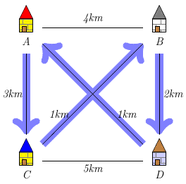
\includegraphics[width=.25\textwidth]{Figures/1. STP/stp.png}};
        
    \node[text width = 0.5\textwidth, right = of logo](title){\sffamily\huge\reporttitle};
    
    \node[text width = 0.5\textwidth, yshift = 0.75cm, below = of title](subtitle){\sffamily\Large \reportsubtitle};
    
    \gettikzxy{(subtitle.south)}{\sffamily\subtitlex}{\subtitley}
    \gettikzxy{(title.north)}{\titlex}{\titley}
    \draw[line width=1mm, Tue-red]($(logo.east)!0.5!(title.west)$) +(0,\subtitley) -- +(0,\titley);
    
    \end{tikzpicture}
    \vspace{3cm}
    
  
    
    \begin{table}[H]
    \centering
    \sffamily
    \large
    \begin{tabu} to 0.8\linewidth {cc}
    \textbf{Etudiant} :  \sffamily\reportauthors
    
    \end{tabu}
    
    \end{table}
    
     \textbf{Professeure:} \sffamily \grouptutor
    
    \tikz[remember picture,overlay]\node[anchor=south,inner sep=0pt] at (current page.south) {
\includegraphics[width=\paperwidth]{Figures/0. General/pied2.jpg}};
    
    \mbox{}
    \vfill
    \iffalse
    \sffamily \Large \textcolor{white}{\placeanddate} \\
    \fi
    
    
    
    \end{titlepage}
    
    
    
    
    
    
    
    
    
\newpage

% Generates a ToC without page number
{\hypersetup{linkcolor=black} % Keeps the ToC black even with non-black linkcolor
	\tableofcontents\thispagestyle{empty}}
\newpage


\section{Présentation du problème}

Le problème du voyageur de commerce \cite{wiki-tsp} peut être défini comme suit :

Soit $G=(V,E)$ un graphe complet, où $V$ est l'ensemble des villes et $E$ est l'ensemble des arêtes pondérées représentant les distances entre les villes. L'objectif est de trouver un cycle hamiltonien $C$ qui visite chaque ville une fois et minimise la somme des distances parcourues.
\newline

Mathématiquement, cela peut être exprimé comme la recherche de la permutation $\pi$ pour minimiser:

$$ d_{Total} = \sum_{i=1}^{n-1}d(\pi(i),\pi(i+1))+d(\pi(n),\pi(1)))$$

où $d(u,v)$) représente la distance entre les villes $u$ et $v$.

\newpage

\section{Instances utilisées}

Nous avons testé notre algorithme sur différentes instances du problème. Ces instances comprennent des graphes complets de petite et grande taille, avec des distances variées entre les villes. Les exemples spécifiques incluent des ensembles de villes générés aléatoirement.
\newline

Nous nous sommes basés sur les 8 asymétriques vue que notre fonction de recharge d'instance le suppose. Tout le code peut bien sûr être utilisé pour les symétriques. Il suffira d'adapter la fonction de recharge. 
\newline

Une instance de nom $atsp\_rand\_X\_Y.txt$ est une instance du problème à $X$ villes avec $Y$ la distance maximale entre deux ville.
\newline

Voici la liste des 8 instances:

\begin{enumerate}
	\item atsp\_rand\_50\_75.txt
	\item atsp\_rand\_50\_100.txt
	\item atsp\_rand\_60\_50.txt
	\item atsp\_rand\_60\_100.txt
	\item atsp\_rand\_70\_55.txt
	\item atsp\_rand\_70\_100.txt
	\item atsp\_rand\_80\_70.txt
	\item atsp\_rand\_80\_100.txt
\end{enumerate}
\newpage

\section{Algorithmes implémentés}
Pour ce TP, nous avons implémenté les différents algorithmes de descente et les recherches locales moins strictes que les
descentes : recherche locale itérée (ILS : Iterated Local Search) et Sampled Walk (SW).

\subsection{Les descentes}
Les algorithmes de descente sont des méthodes heuristiques qui visent à améliorer itérativement une solution initiale en explorant son voisinage. Les algorithmes de descente peuvent être classés en différentes catégories en fonction de la relation de voisinage et de la manière dont ils choisissent le voisin. Les trois principaux types d'algorithmes de descente sont le meilleur voisin, le premier améliorant et le pire voisin.

\subsubsection{Les relation de voisinage}
\begin{itemize}
	\item Swap : elle consiste à échanger les positions de deux villes dans le parcours du voyageur.
	\item 2-opt : elle  consiste à inverser l'ordre des villes entre deux positions du parcours du voyageur.
\end{itemize}

\subsubsection{Choix de voisin}
\begin{itemize}
	\item Meilleur améliorant
	
	L'algorithme du meilleur améliorant (Algo~\ref{algo:meilleur_aml}) explore tous les voisins d'une solution et sélectionne celui qui offre la meilleure amélioration en termes de fonction objectif.
	
	Dans les pseudos codes nous tenons seulement compte des arguments importants pour la compréhension.
	
	\begin{algorithm}[H]
		\caption{Meilleur améliorant}
		\label{algo:meilleur_aml}
		\begin{algorithmic}[1]
			\Require{$ voisins  = $ voisins générés avec swap ou 2-opt}
			\Require{$solution$ : solution actuelle}
			\Ensure{$meilleur\_voisin$}
			\Statex
			
			\Function{best\_improver}{$\mathbf{solution}$, $\mathbf{voisins}$}
			\State {$meilleur\_voisin$ $\gets$ {$NULL$}}
			\State {$cur\_cost$ $\gets$ {$cost(solution)$}}

			\For { \textbf{each} $voisin$ \textbf{in}
				 $voisins$}                    
			\If{$cost(voisin) < cur\_cost$}  
				\State {$meilleur\_voisin$ $\gets$ {$voisin$}}
				\State {$cur\_cost$ $\gets$ {$cost(voisin)$}}
			\EndIf
			\EndFor
			\State \Return {$meilleur\_voisin$}
			\EndFunction
			
		\end{algorithmic}
	\end{algorithm}
	
	\item Premier améliorant
	
	Contrairement à l'algorithme du meilleur améliorant, l'algorithme du premier améliorant (Algo ~\ref{algo:first_improver}) s'arrête dès qu'il trouve le premier voisin qui améliore la solution courante.
	
		\begin{algorithm}[H]
		\caption{Premier améliorant}
		\label{algo:first_improver}
		\begin{algorithmic}[1]
			\Require{$ voisins  = $ voisins générés avec swap ou 2-opt}
			\Require{$solution$ : solution actuelle}
			\Ensure{$premier\_ameliorant$}
			\Statex
			
			\Function{first\_improver}{$\mathbf{solution}$, $\mathbf{voisins}$}
			\State {$cur\_cost$ $\gets$ {$cost(solution)$}}
			
			\For { \textbf{each} $voisin$ \textbf{in}
				$voisins$}                    
			\If{$cost(voisin) < cur\_cost$}  
			\State \Return {$voisin$}
			\EndIf
			\EndFor
		\State \Return {$NULL$}
			\EndFunction
			
		\end{algorithmic}
	\end{algorithm}
	
	\item Pire améliorant
	L'algorithme du pire améliorant (Algo ~\ref{algo:worst_improver}) explore tous les voisins d'une solution et sélectionne celui qui offre la pire amélioration.
	
		\begin{algorithm}[H]
		\caption{Pire améliorant}
		\label{algo:worst_improver}
		\begin{algorithmic}[1]
			\Require{$ voisins  = $ voisins générés avec swap ou 2-opt}
			\Require{$solution$ : solution actuelle}
			\Ensure{$pire\_voisin$}
			\Statex
			
			\Function{worst\_improver}{$\mathbf{solution}$, $\mathbf{voisins}$}
			\State {$meilleur\_voisin$ $\gets$ {$NULL$}}
			\State {$cur\_cost$ $\gets$ {$-1 $}}
			
			\For { \textbf{each} $voisin$ \textbf{in} $voisins$}    
			                
			\If{$cost(voisin) < cost(solution)  $ \textbf{and}  $cost(voisin) > cur\_cost$  }  
			\State {$pire\_voisin$ $\gets$ {$voisin$}}
			\State {$cur\_cost$ $\gets$ {$cost(voisin)$}}
			\EndIf
			\EndFor
			\State \Return {$pire\_voisin$}
			\EndFunction
			
		\end{algorithmic}
	\end{algorithm}
	
\end{itemize}

En utilisant les deux relations de voisinage pour chacun on six algos de choix de voisin pour la descente :
\begin{enumerate}
	\item best\_improver\_swap
	\item first\_improver\_swap
	\item worst\_improver\_swap
	\item best\_improver\_2opt
	\item first\_improver\_2opt
	\item worst\_improver\_2opt
\end{enumerate}

\subsubsection{Descente complète}
On part d’une solution initiale. Tant que la solution courante n’est pas un optimum local, on génère un voisin selon le couple (voisinage, pivot) pour remplacer la solution courante. Voici son pseudo code Aglo~\ref{algo:descente} :

	\begin{algorithm}[H]
	\caption{Descente complète}
	\label{algo:descente}
	\begin{algorithmic}[1]
		\Require{$algo$ : l'un de 6 algo de choix de voisin}
		\Require{$solution$ : solution initiale}
		\Ensure{$solution\_final$}
		\Statex
		
		\Function{descente}{$\mathbf{solution}$, $\mathbf{algo}$}
		\State {$solution\_final$ $\gets$ {$solution$}}
		\State {$voisins$ $\gets$ {$generate\_voisins(solution)$}} \Comment{avec swap ou 2-opt selon le cas}
		\State {$new\_solution$ $\gets$ {$algo(solution,voisins)$}}
		
		\While{$new\_solution != NULL$}
			\State {$solution\_final$ $\gets$ {$new\_solution$}}
			\State {$voisins$ $\gets$ {$generate\_voisins(solution\_final)$}}
			\State {$new\_solution$ $\gets$ {$algo(solution\_final,voisins)$}}
		\EndWhile
		
		\State \Return {$solution\_final$}
		\EndFunction
		
		
	\end{algorithmic}
\end{algorithm}

\subsection{Iterated Local Search(ILS)}
ILS (Algo~\ref{algo:ils}) utilise la descente. A chaque fin de descente, tant que le critère d’arrêt n’est pas atteint un nombre de perturbations sera appliqué à la meilleure solution rencontrée depuis le début de l’exécution. En fin d’exécution
la solution retournée sera la meilleure rencontrée. 


Le critère d'arrêt utilisé est le nombre d’évaluation maximal.

\begin{algorithm}[H]
	\caption{ILS}
	\label{algo:ils}
	\begin{algorithmic}[1]
		\Require{$solution$ : solution initiale}
		\Require{$algo$ : l'un de 6 algo de choix de voisin}
		\Require{$nb\_pertubations$ : nombre de perturbations}
		\Require{$max\_eval$ : nombre d’évaluation maximal}
		\Ensure{$best\_sol$}
		\Statex
		
		\Function{ils}{$\mathbf{solution}$, $\mathbf{algo}$, $\mathbf{nb\_pertubations}$, $\mathbf{max\_eval}$}
		
		\State {$nombre\_evaluations$ $\gets$ {$0$}} \Comment{Variable globale, incrémentée à chaque évaluation}
		
		\State {$best\_sol$ $\gets$ {$solution$}}
		\State {$cur\_sol$ $\gets$ {$solution$}}
	
		\While{$nombre\_evaluations < max\_eval$}
		\State {$new\_sol$ $\gets$ {$descente(cur\_sol,algo)$}}
		\If{$cost(new\_sol) < cost(best\_sol)$}
			\State {$best\_sol$ $\gets$ {$new\_sol$}}
		\EndIf  
		\State {$cur\_sol$ $\gets$ {$apply\_pertubations(best\_sol,nb\_pertubations)$}}
		\EndWhile
		
		\State \Return {$best\_sol$}
		\EndFunction
		
		
	\end{algorithmic}
\end{algorithm}



\subsection{Sampled Walk (SW)}
SW (Algo~\ref{algo:sw}) est une recherche locale dont le principe est de générer $\lambda$ voisins à chaque étape de la recherche et de sélectionner celui au meilleur score.
Le critère d'arrêt utilisé est le nombre d’évaluation maximal.

\begin{algorithm}[H]
	\caption{SW}
	\label{algo:sw}
	\begin{algorithmic}[1]
		\Require{$solution$ : solution initiale}
		\Require{$\lambda$ : nombre de voisins à générer }
		\Require{$max\_eval$ : nombre d’évaluation maximal}
		\Ensure{$best\_sol$}
		\Statex
		
		\Function{sw}{$\mathbf{solution}$, $\mathbf{algo}$, $\mathbf{nb\_pertubations}$, $\mathbf{max\_eval}$}
		
		\State {$nombre\_evaluations$ $\gets$ {$0$}} \Comment{Variable globale, incrémentée à chaque évaluation}
		
		\State {$best\_sol$ $\gets$ {$solution$}}
		
		
		\While{$nombre\_evaluations < max\_eval$}
		\State {$new\_sol$ $\gets$ {$generate\_and\_choice\_best(best\_sol,\lambda)$}}
		\If{$cost(new\_sol) < cost(best\_sol)$}
		\State {$best\_sol$ $\gets$ {$new\_sol$}}
		\EndIf  
		\EndWhile
		
		\State \Return {$best\_sol$}
		\EndFunction
		
		
	\end{algorithmic}
\end{algorithm}

\subsection{Algorithme génétique : Bonus}
J'ai choisi de faire l'algorithme génétique pour varier comme on a fait que des recherches. locales.
\newline
De façon générale un algorithme génétique pour la résolution d’un problème d’optimisation fonctionne sur le principe suivant.
\begin{itemize}
	\item \textbf{Création de la Population Initiale} :

Génération d'un groupe d'individus représentant différentes solutions possibles.

\item \textbf{Sélection des Parents }:

Choix d'individus parents, souvent basé sur leur performance (fitness).

\item \textbf{Croisement (Crossover) }:

Les parents se reproduisent en échangeant une partie de leurs caractéristiques pour créer des enfants.

\item \textbf{Mutation :}

Les enfants peuvent subir des modifications aléatoires pour introduire de la diversité.

\item \textbf{Sélection des Survivants (Fitness) :}

Évaluation de la performance de la population totale et sélection des individus les plus adaptés pour survivre.

\item \textbf{Itération }:

Répétition des étapes de reproduction, mutation, et sélection sur plusieurs générations.
\end{itemize}

\newpage

\section{Protocole expérimental}

Pour comparer les méthodes par la suite, nous avons fait plusieurs exécutions
par méthode. 

\begin{itemize}
	\item Pour les descentes
	
	Nous somme partis de 10 solutions initiales différentes. Pour chaque triplet (instance, algo de descente, solution initiale), nous avons fait une exécution. Donc au total 8x6x10=480 exécutions.  Nous avons utilisé des $seeds$ (10 seeds) pour la gestion des solutions initiales. 
	
	Le score des optima et les temps d'exécution sont conservé dans un fichier csv d'entête : 
	$Instance,Algorithme,Seed,Score,CPU-Used-Time (ms)$
	
	\item Pour ILS et SW
	
	Nous somme partis de 10 solutions initiales différentes, de deux valeurs de nombre de perturbations et de $\lambda$ et utilisé la même valeur pour nombre d’évaluation maximal.
	
	\begin{itemize}
		\item ILS : une exécution par (instance, algo ISL, solution initiale, nb perturbation)
		
		8*4*10*2 = 640
		
		Entête CSV : $Instance,Algorithme,Seed,Score,NbPertubations,MaxEval,CPU-Used-Time (ms)$
		
		\item SW : une exécution par (instance, algo SW, solution initiale, lambda)
		
		8*2*10*2 = 320
		
		
		Entête CSV : $Instance,Algorithme,Seed,Score,Lambda,MaxEval,CPU-Used-Time (ms)$
	\end{itemize}
	
	
\end{itemize}

\newpage

\section{Résultats obtenus}

\subsection{Descentes}
\subsubsection{Résultats des versus}
Les deux tableaux suivants présentent combien de fois sur 10 exécution une méthode gagne contre l'autre. 

Pour methode1\_vs\_methode2, $(n_1,n_2)$ signifie que methode1 gagne $n_1$ fois et methode2 gagne $n_2$ fois. Évidemment $n_1+n_2=10$.
\iffalse
\begin{table}[ht]
	\rowcolors{2}{gray!10}{white}
	\centering
	\caption{list of symbols}
	\begin{tabular}[t]
		{m{0.1\textwidth}m{0.25\textwidth}m{0.25\textwidth}m{0.2\textwidth}}
		\toprule
		\textbf{Symbol}&\textbf{dimension}&\textbf{Unit}&\textbf{Unit abbreviation}\\
		\midrule
		1&2&3&4\\
		1&2&3&4\\
		1&2&3&4\\
		1&2&3&4\\
		\bottomrule
	\end{tabular}

\end{table}


\begin{table}[ht]
	\rowcolors{2}{gray!10}{white}
	\centering
	\caption{Nombre de fois qu'une méthode gagne contre l'autre}
		\begin{tabular}[t]
			{m{0.2\textwidth}m{0.2\textwidth}m{0.2\textwidth}m{0.2\textwidth} m{0.2\textwidth} m{0.2\textwidth}m{0.2\textwidth}}
			\toprule
	instances &	swap\_first\_vs\_best&	swap\_first\_vs\_worst &	swap\_best\_vs\_worst&	2opt\_first\_vs\_best&	2opt\_first\_vs\_worst&	2opt\_best\_vs\_worst\\
	\midrule
	rand\_50\_75.txt&	(6, 4)&	(5, 5)&	(4, 6)&	(7, 3)&	(8, 2)&	(6, 4)\\
	rand\_50\_100.txt&	(5, 5)&	(6, 4)&	(5, 5)&	(9, 1)&	(10, 0)&	(7, 3)\\
	rand\_60\_50.txt&	(4, 6)&	(3, 7)&	(5, 5)&	(8, 2)&	(10, 0)&	(7, 3)\\
	rand\_60\_100.txt&	(4, 6)&	(5, 5)&	(5, 5)&	(9, 1)&	(10, 0)&	(7, 3)\\
	rand\_70\_55.txt&	(7, 3)&	(4, 6)&	(5, 5)&	(10, 0)&	(8, 2)&	(3, 7)\\
	rand\_70\_100.txt&	(5, 5)&	(6, 4)&	(4, 6)&	(9, 1)&	(10, 0)&	(5, 5)\\
	rand\_80\_70.txt&	(3, 7)&	(5, 5)&	(3, 7)&	(10, 0)&	(10, 0)&	(5, 5)\\
	rand\_80\_100.txt&	(6, 4)&	(5, 5)&	(5, 5)&	(9, 1)	&(10, 0)&	(4, 6)\\
	\bottomrule
\end{tabular}
\end{table}
\fi
\begin{table}[ht]
	\rowcolors{2}{gray!10}{white}
	\centering
	\caption{Nombre de fois qu'une méthode gagne contre l'autre (swap)}
	\begin{tabular}[t]
		{m{0.2\textwidth}m{0.2\textwidth}m{0.2\textwidth}m{0.2\textwidth}}
		\toprule
		instances &	swap\_first\_vs\_best&	swap\_first\_vs\_worst &	swap\_best\_vs\_worst\\
		\midrule
		rand\_50\_75.txt&	(6, 4)&	(5, 5)&	(4, 6)\\
		rand\_50\_100.txt&	(5, 5)&	(6, 4)&	(5, 5)\\
		rand\_60\_50.txt&	(4, 6)&	(3, 7)&	(5, 5)\\
		rand\_60\_100.txt&	(4, 6)&	(5, 5)&	(5, 5)\\
		rand\_70\_55.txt&	(7, 3)&	(4, 6)&	(5, 5)\\
		rand\_70\_100.txt&	(5, 5)&	(6, 4)&	(4, 6)\\
		rand\_80\_70.txt&	(3, 7)&	(5, 5)&	(3, 7)\\
		rand\_80\_100.txt&	(6, 4)&	(5, 5)&	(5, 5)\\
		\bottomrule
	\end{tabular}
\end{table}

\begin{table}[ht]
	\rowcolors{2}{gray!10}{white}
	\centering
	\caption{Nombre de fois qu'une méthode gagne contre l'autre (2opt)}
	\begin{tabular}[t]
		{m{0.2\textwidth}m{0.2\textwidth}m{0.2\textwidth}m{0.2\textwidth} m{0.2\textwidth} m{0.2\textwidth}m{0.2\textwidth}}
		\toprule
		instances &		2opt\_first\_vs\_best&	2opt\_first\_vs\_worst&	2opt\_best\_vs\_worst\\
		\midrule
		rand\_50\_75.txt&		(7, 3)&	(8, 2)&	(6, 4)\\
		rand\_50\_100.txt&		(9, 1)&	(10, 0)&	(7, 3)\\
		rand\_60\_50.txt&		(8, 2)&	(10, 0)&	(7, 3)\\
		rand\_60\_100.txt&		(9, 1)&	(10, 0)&	(7, 3)\\
		rand\_70\_55.txt&		(10, 0)&	(8, 2)&	(3, 7)\\
		rand\_70\_100.txt&		(9, 1)&	(10, 0)&	(5, 5)\\
		rand\_80\_70.txt&	    (10, 0)&	(10, 0)&	(5, 5)\\
		rand\_80\_100.txt&		(9, 1)	&(10, 0)&	(4, 6)\\
		\bottomrule
	\end{tabular}
\end{table}

\subsubsection{Moyenne des scores}
En prenant la moyenne des scores, on a :  

\begin{table}[ht]
	\rowcolors{2}{gray!10}{white}
	\centering
	\caption{Moyenne des scores}
	\begin{tabular}[t]
		{m{0.2\textwidth}m{0.2\textwidth}m{0.2\textwidth}m{0.2\textwidth} }
		\toprule
		 &		first&	worst&	best\\
		\midrule
		swap&		1205.8250&	1207.7250&	1206.7625\\
		2opt&		1596.2125&1809.1750 &	1801.5000\\
	
		\bottomrule
	\end{tabular}
\end{table}

On constate que dans le deux cas, \textbf{first} semble être la meilleur méthode.

%On peut aussi déduire des deux premiers tableaux que\textbf{ first} gagne \textbf{115} fois contre \textbf{worst} et\textbf{ worst} seulement \textbf{45} fois contre \textbf{first}. 
\subsubsection{Durée et influence de l'évaluation incrémentale}
Le tableau suivant résume la durée moyenne des \textbf{descentes swap} avec et sans l'évaluation incrémentale (EI).
\begin{table}[ht]
	\rowcolors{2}{gray!10}{white}
	\centering
	\caption{Moyenne des durées en ms}
	\begin{tabular}[t]
		{m{0.2\textwidth}m{0.2\textwidth}m{0.2\textwidth}m{0.2\textwidth} }
		\toprule
		&best\_improver&	first\_improver&	wors\_improver\\
		\midrule
		sans EI &		23.713987&	7.646788&	885.963613\\
		avec EI &		4.497738& 0.354200 &	50.475100\\
		
		\bottomrule
	\end{tabular}
\end{table}

Il en ressort que \textbf{first} est plus rapide que \textbf{best} qui est plus rapide que \textbf{worst}. On remarque aussi que l'\textbf{évaluation incrémentale} a considérablement améloré la rapidité. 


\subsection{ILS et SW}

\subsubsection{ILS}
\begin{itemize}
	\item \textbf{Résultats des versus}
	
	Le tableau suivant présente combien de fois sur 20 exécutions (deux valeurs pour nombre de perturbations) une méthode gagne contre l'autre. 
	
	\begin{table}[ht]
		\rowcolors{2}{gray!10}{white}
		\centering
		\caption{Nombre de fois qu'une méthode gagne contre l'autre}
		\begin{tabular}[t]
			{m{0.2\textwidth}m{0.2\textwidth}m{0.2\textwidth}}
			\toprule
			instances &	swap\_first\_vs\_best &	2opt\_first\_vs\_best \\
			
			\midrule
			rand\_50\_75.txt&	(11, 9)	&(15, 5)\\
			rand\_50\_100.txt&	(5, 15)&	(19, 1)\\
			rand\_60\_50.txt&	(11, 9)&	(17, 3)\\
			rand\_60\_100.txt&	(6, 14)&	(18, 2)\\
			rand\_70\_55.txt&	(9, 11)&	(18, 2)\\
			rand\_70\_100.txt&	(13, 7)	&(20, 0)\\
			rand\_80\_70.txt&	(10, 10)	&	(18, 2)\\
			rand\_80\_100.txt&	(10, 10)	&	(18, 2)\\
			
		
			\bottomrule
		\end{tabular}
	\end{table}
\item \textbf{Moyenne des scores}

\begin{table}[ht]
	\rowcolors{2}{gray!10}{white}
	\centering
	\caption{Moyenne des scores}
	\begin{tabular}[t]
		{m{0.2\textwidth}m{0.2\textwidth}m{0.2\textwidth}}
		\toprule
		méthode &		first&		best\\
		\midrule
		swap&		1163.11250&	1161.33750\\
		2opt&		1496.33125& 1654.21875 \\
		
		\bottomrule
	\end{tabular}
\end{table}
On constate que \textbf{first} domine \textbf{best} pour 2opt mais pas pour swap.
\end{itemize}


\subsubsection{SW}
\begin{itemize}
	\item \textbf{Résultats des versus}
	
	Le tableau suivant présente combien de fois sur 20 exécutions (deux valeurs pour nombre de perturbations) une méthode gagne contre l'autre. 
	
	\begin{table}[H]
		\rowcolors{2}{gray!10}{white}
		\centering
		\caption{Nombre de fois qu'une méthode gagne contre l'autre}
		\begin{tabular}[t]
			{m{0.2\textwidth}m{0.2\textwidth}}
			\toprule
			instances &	swap\_vs\_2opt  \\
			
			\midrule
			rand\_50\_75.txt& (20, 0)	\\
			rand\_50\_100.txt& (20, 0)	\\
			rand\_60\_50.txt& (20, 0)	\\
			rand\_60\_100.txt& (20, 0)	\\
			rand\_70\_55.txt&	(20, 0)\\
			rand\_70\_100.txt&	(20, 0)\\
			rand\_80\_70.txt&(20, 0)	\\
			rand\_80\_100.txt&	(20, 0)\\
			
			
			\bottomrule
		\end{tabular}
	\end{table}
	\item \textbf{Moyenne des scores}
	
	\begin{table}[ht]
		\rowcolors{2}{gray!10}{white}
		\centering
		\caption{Moyenne des scores}
		\begin{tabular}[t]
			{m{0.2\textwidth}m{0.2\textwidth}m{0.2\textwidth}}
			\toprule
			 &		Moyenne\\
			\midrule
			swap&		1209.74375 \\
			2opt&		1818.96875\\
			
			\bottomrule
		\end{tabular}
	\end{table}
	On constate que \textbf{swap} domine \textbf{2opt}.
\end{itemize}
\newpage

\section{Conclusion}
L'analyse des performances des descentes, des algorithmes de recherche locale moins strictes, a fourni des résultats significatifs. Voici quelques observations clés :

\begin{itemize}
	\item La descente \textbf{first} s'est avérée plus rapide et plus performante que \textbf{best} et \textbf{worst} dans l'ensemble.


\item La relation de voisinage \textbf{swap} a montré une performance parfois supérieure à celle de \textbf{2-opt}.


\item L'introduction de l'évaluation incrémentale a considérablement amélioré la rapidité des algorithmes en réduisant le nombre d'évaluations nécessaires. L'évaluation incrémentale offre une approche efficace pour économiser des ressources.

\item Dans le contexte d'ILS, la stratégie \textbf{first} a aussi montré une domination par rapport à d'autres approches.


\item L'algorithmes génétique a montré de bons résultats en termes de qualité des solutions obtenues. L'efficacité de l'algorithme génétique peut être influencée par la taille de la population, la probabilité de croisement, et d'autres paramètres.

\end{itemize}
En conclusion, il n'y a pas d'approche unique qui fonctionne le mieux dans tous les cas. Le choix de l'algorithme et des heuristiques dépend fortement des caractéristiques spécifiques du problème. Une approche expérimentale peut aider à identifier les stratégies les plus performantes dans des contextes variés. Les résultats obtenus suggèrent que des techniques telles que la descente \textbf{first}, le voisinage \textbf{swap},  peuvent être des choix prometteurs selon le contexte du problème étudié.
\newline

Le code est aussi disponible sur mon github :
\href{}{https://github.com/dinyad-prog00/TSP--traveling-salesman-problem} 



\newpage



% Creates references using the Biblatex 
%\bibliographystyle{plain}
%\bibliography{General/References.bib}

\nocite{*}
\printbibliography[title=Bibliographie]

\newpage


\end{document}
